\documentclass[11pt,a4paper]{article}

\usepackage[a4paper,margin=1in]{geometry}
\usepackage[T1]{fontenc}
\usepackage[utf8]{inputenc}
\usepackage{lmodern}
\usepackage{array}
\usepackage{booktabs}
\usepackage{float}
\usepackage{graphicx}
\usepackage{titling}
\usepackage{tabularx}
\usepackage{enumitem}
\usepackage{hyperref}

\hypersetup{
  colorlinks=true,
  linkcolor=blue,
  urlcolor=blue,
  citecolor=blue
}

\setlength{\parskip}{0.6em}
\setlength{\parindent}{0pt}
\renewcommand{\arraystretch}{1.2}
\newcolumntype{Y}{>{\raggedright\arraybackslash}X}

\title{Digit Recognition with LeNet-5 on MNIST}
\author{Nandu Krishna M 25CSE2015}
\date{\today}

\begin{document}

\begin{center}
{\Huge\bfseries ANN ASSIGNMENT\par}
\vspace{0.25em}
{\Large \thetitle\par}
\vspace{0.35em}
{\normalsize \theauthor\par}
{\normalsize GitHub repository: \href{https://github.com/TheGhossst/ann-assignment}{ann-assignment}\par}
\vspace{0.15em}
{\normalsize \thedate\par}
\end{center}
\vspace{-0.75em}

\section{Dataset}
The dataset used in this project is MNIST, a standard benchmark for handwritten digit recognition. The program loads it through \texttt{torchvision.datasets.MNIST} with separate training and test splits. In the code, the dataset contains 70,000 images in total:
\begin{itemize}[leftmargin=*]
  \item 60,000 training images
  \item 10,000 test images
\end{itemize}
Each image belongs to one of 10 classes, representing digits 0 through 9. Every sample is a 28$\times$28 grayscale image, which the program converts into a 1$\times$28$\times$28 tensor for the CNN. If flattened, each image contains 784 pixel values.

\begin{table}[h]
\centering
\caption{MNIST dataset summary}
\begin{tabular}{ll}
\toprule
Property & Value \\
\midrule
Total images & 70,000 \\
Training images & 60,000 \\
Test images & 10,000 \\
Number of classes & 10 \\
Image size & 28$\times$28 grayscale \\
Program input tensor & 1$\times$28$\times$28 \\
Flattened pixel values & 784 \\
\bottomrule
\end{tabular}
\end{table}

\section{LeNet-5 Model}
LeNet-5 is one of the earliest and most influential convolutional neural network architectures for digit classification. In this project, it is adapted for MNIST by using one grayscale input channel and a padded first convolution so the spatial size remains 28$\times$28 before pooling.

\begin{figure}[H]
\centering
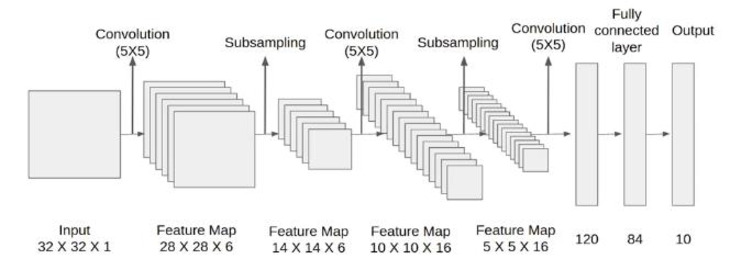
\includegraphics[width=0.95\linewidth]{../images/letnet5.jpg}
\caption{LeNet-5 CNN architecture reference used for the project report.}
\label{fig:lenet-5-architecture}
\end{figure}

\begin{table}[H]
\centering
\caption{Model architecture used in the project}
\begin{tabularx}{\textwidth}{lYc}
\toprule
Layer & Configuration / Output & Parameters \\
\midrule
Input & 1$\times$28$\times$28 grayscale image tensor & 0 \\
Conv1 & 6 filters, 5$\times$5 kernel, padding 2, Tanh; output 6$\times$28$\times$28 & 156 \\
Pool1 & Average pooling, 2$\times$2, stride 2; output 6$\times$14$\times$14 & 0 \\
Conv2 & 16 filters, 5$\times$5 kernel, Tanh; output 16$\times$10$\times$10 & 2,416 \\
Pool2 & Average pooling, 2$\times$2, stride 2; output 16$\times$5$\times$5 & 0 \\
Conv3 & 120 filters, 5$\times$5 kernel, Tanh; output 120$\times$1$\times$1 & 48,120 \\
Flatten & Reshape to a 120-dimensional vector & 0 \\
FC1 & Linear 120$\rightarrow$84, Tanh; output 84 & 10,164 \\
Output & Linear 84$\rightarrow$10 logits, one per digit class & 850 \\
\bottomrule
\end{tabularx}
\end{table}

The network has 61,706 trainable parameters. It is trained with Adam, batch size 64, learning rate 0.001, weight decay 1e-4, and a step learning-rate scheduler.

\section{Observations}
\begin{enumerate}[leftmargin=*]
  \item The model classified the clearer digits very confidently, with several predictions close to 100\% confidence.
  \item Digits 4 and 6 were more difficult because their handwriting styles were less distinct than the simpler digits.
  \item The model confused 4 with 8 and 9 with 7, which shows that similar stroke patterns can lead to misclassification.
  \item The preprocessing pipeline is important: grayscale conversion, inversion, cropping, padding, resizing, and normalization make custom images more consistent with MNIST.
  \item Even with a compact size of 61,706 parameters, LeNet-5 achieved strong performance on handwritten digit recognition, which makes it a good lightweight CNN baseline.
\end{enumerate}

The custom image files are named by their true labels, so 0.png corresponds to class 0, 1.png to class 1, and so on.

\begin{table}[h]
\centering
\caption{Inference results on custom images}
\begin{tabular}{lrrr}
\toprule
Image & Actual class & Predicted class & Confidence \\
\midrule
0.png & 0 & 0 & 99.99\% \\
1.png & 1 & 1 & 99.99\% \\
2.png & 2 & 2 & 99.89\% \\
3.png & 3 & 3 & 100.00\% \\
4.png & 4 & 8 & 62.25\% \\
5.png & 5 & 5 & 99.98\% \\
6.png & 6 & 6 & 73.87\% \\
7.png & 7 & 7 & 98.86\% \\
8.png & 8 & 8 & 100.00\% \\
9.png & 9 & 7 & 99.95\% \\
\bottomrule
\end{tabular}
\end{table}

\section{Conclusion}
This project demonstrates that a LeNet-5 style convolutional neural network is effective for MNIST digit recognition. The dataset is simple enough for a compact model, yet it still reveals where ambiguity in handwriting can challenge the classifier. The results show that the model is highly reliable on most digits, while a few visually similar samples remain difficult cases.

\end{document}